% Copyright 2020-2024 Richard J. Zak
% richard.j.zak@gmail.com

\documentclass[letter,10pt]{article}
\usepackage[breaklinks]{hyperref}
\hypersetup{
    bookmarks=true,         % show bookmarks bar?
    unicode=false,          % non-Latin characters in Acrobat’s bookmarks
    pdftoolbar=true,        % show Acrobat’s toolbar?
    pdfmenubar=true,        % show Acrobat’s menu?
    pdffitwindow=false,     % window fit to page when opened
    pdfstartview={XYZ null null 1.00},    % disable zoom
    pdftitle={Project 2},    % title
    pdfauthor={Richard Zak},     % author
    pdfsubject={UMBC CMSC104 Problem Solving and Computer Programming},   % subject of the document
    pdfkeywords={Computer Science, Programming, Problem Solving, CSEE}, % list of keywords
    pdfnewwindow=true,      % links in new PDF window
    colorlinks=false,       % false: boxed links; true: colored links
    linkcolor=red,          % color of internal links (change box color with linkbordercolor)
    citecolor=green,        % color of links to bibliography
    filecolor=magenta,      % color of file links
    urlcolor=cyan           % color of external links
}
\usepackage{graphicx}
\usepackage{fancyhdr}
\usepackage{multicol}
\pagestyle{fancy}
\usepackage[letterpaper, margin=1in]{geometry}
\geometry{letterpaper}
\usepackage{listings} % Syntax highlighing
\usepackage{xcolor}
\usepackage{parskip} % Disable initial indent
\usepackage{color,soul} % Highligher
\usepackage[normalem]{ulem} % Strikethrough with \sout{}

\definecolor{codegreen}{rgb}{0,0.6,0}
\definecolor{codegray}{rgb}{0.5,0.5,0.5}
\definecolor{codepurple}{rgb}{0.58,0,0.82}
\definecolor{backcolour}{rgb}{0.97,0.97,0.97}

\lstdefinestyle{mystyle}{
    backgroundcolor=\color{backcolour},
    commentstyle=\color{codegreen},
    keywordstyle=\color{magenta},
    numberstyle=\tiny\color{codegray},
    stringstyle=\color{codepurple},
    basicstyle=\ttfamily\small,
    breakatwhitespace=false,
    breaklines=true,
    captionpos=b,
    keepspaces=true,
    numbers=left,
    numbersep=5pt,
    showspaces=false,
    showstringspaces=false,
    showtabs=false,
    tabsize=2
}

\lstset{style=mystyle}

\usepackage[utf8]{inputenc}
\fancyhf{}
\renewcommand{\headrulewidth}{0pt} % Remove default underline from header package
\rhead{CMSC 104 Section 01: Project 2}
%\rhead{}
\lhead{\begin{picture}(0,0) \put(0,-10){
\includegraphics[width=1.1cm]{../../Images/UMBC-vertical}} \end{picture}}
\cfoot{\thepage}
\rfoot{Fall 2024
}
\lfoot{CMSC 104 Section 01}
\AtEndDocument{\vfill \footnotesize{Last modified: 03 August 2024}}
\AtEndDocument{\rfoot{Fall 2024
}}
\renewcommand\thesubsection{\arabic{subsection}} % Show only subsection numbers, not section.subsection

\begin{document}
    
    \huge
    \textbf{Project 2: The Emojifier!}
    \normalsize
    \\ ~~ \\
    \textbf{In-class Date: ASSIGNED} \\
    \textbf{Due Date: DUE}
    
    \section*{Objectives}
    \paragraph{}To create a program which receives sentences (or longer) and inserts emoji icons in the correct location.
    
    \section*{Background}
    \paragraph{}As discussed in Chapter 5, strings are a collection of individual characters. For most characters, specially in European languages, the ASCII table is used (visit \url{https://www.asciitable.com/}). It shows the mapping between a number and a character. For example, the integer 65 is a capital `A', and the integer 48 represents the number zero when shown in a string. The ASCII table only allows for 256 possible values, and there are a lot more than 256 different characters to be displayed when considering the world's many languages! For that, there's Unicode. Part of Unicode also encodes for emojis. The full list of all emoji characters and the byte sequences that produce them are available at \url{https://unicode.org/emoji/charts/full-emoji-list.html}.
    
    \subsection*{Assignment}
    \paragraph{}Using the starter code below, 
    
    \begin{lstlisting}[language=python]
# Name: Alice Smith (your name here!)

emoji = {
    'happy': "\U0001F600",
}

user_input = ???

for fragment in user_input.split():
    # If 'fragment' is in 'emoji', replace 'fragment' with 'emoji[fragment]'
    ???

print(user_input)
    \end{lstlisting}

    \subsubsection*{Notes}
    \paragraph{}To prevent Python from misinterpreting the emoji bytes or from returning an error:
    \begin{enumerate}
        \item The emoji codes are all four bytes in length (\texttt{0x00, 0x01, 0xF6, 0x00}, you'll need leading zeroes).
        \item The bytes must be in quotes.
        \item The bytes must start with \texttt{\textbackslash U}.
    \end{enumerate}
    \paragraph{}In addition, ensure to handle punctuation, such as ``happy'' vs. ``happy\textbf{,}''.
    
    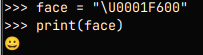
\includegraphics{proj2_python_face}
    
    \section*{Reminder}
    \paragraph{}Assignments are your own effort. Do not share your code.
    
    \section*{Extra Credit}
    \paragraph{}Add aliases, so two or more words may map to the same emoji without having the emoji code duplicated.
    
    \section*{Grading Rubric}
    \paragraph{}Script prints:
    \begin{itemize}
        \item Program works: 75 points.
        \item At least 100 Emojis: 25 points.
        \begin{itemize}
            \item Extra credit: +10 points.
        \end{itemize}
    \end{itemize}
    
    \section*{What to Submit}
    \begin{itemize}
        \item Your Python script.
    \end{itemize}
    
\end{document}
